\textbf{Visualization.} To analyze the behaviour of the models, we propose visualizations of the evolutions of the parameters predicted by \DirModel and \GPModel.

\textit{Set-up:} We use two toy datasets where the probability of an event depends only on time. The first one (\textbf{3-G}) has three classes occuring at three distinct times. It represents the events in the Fig.\ \ref{fig:car_categorical}. The second one (\textbf{Multi-G}) consists of two classes where one of them has two modes and corresponds to the Fig.\ \ref{fig:kitchen_categorical}. We use these datasets to showcase the importance of time when predicting the next event. In Fig.\ \ref{fig:visualization}, the four top plots show the evolution of the categorical distribution for the \DirModel and the logits for the \GPModel with $10$ points each. The four bottom plots describe the certainty of the models on the probability prediction by plotting the probability $q_\IndexClass(\DeltaTime)$ that the probability of class $\IndexClass$ is higher than others, as introduced in Sec.\ \ref{model_description}.
% These values are computed with sampling methods for \DirModel and with a closed-form expression for \GPModel which explains the difference in the smoothness of these curves.
Additionally, the evolution of the dirichlet distribution over the probability simplex is presented in Appendix \ref{dirichlet_triangle_evolution}.

\begin{figure}
\centering
    \begin{subfigure}{.24\textwidth}
        \centering
        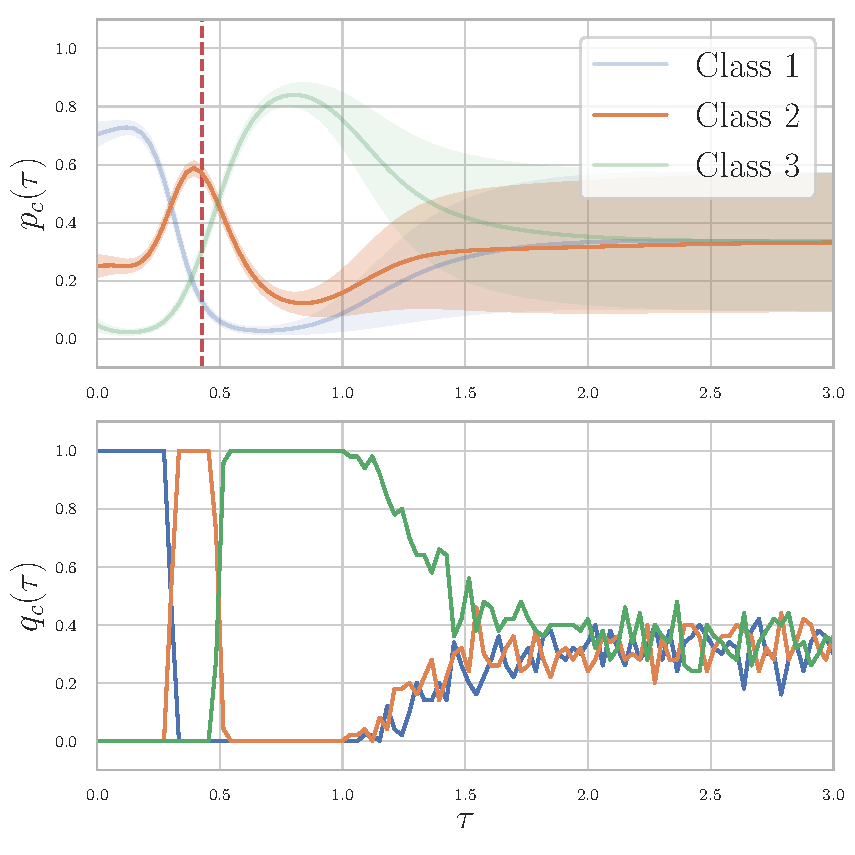
\includegraphics[width=\linewidth]{sections/010_neurips2019/paper/images/shifted-gaussians-dirichlet.pdf}
        \caption*{\DirModel on 3-G}
    \end{subfigure}
    \begin{subfigure}{.24\textwidth}
        \centering
        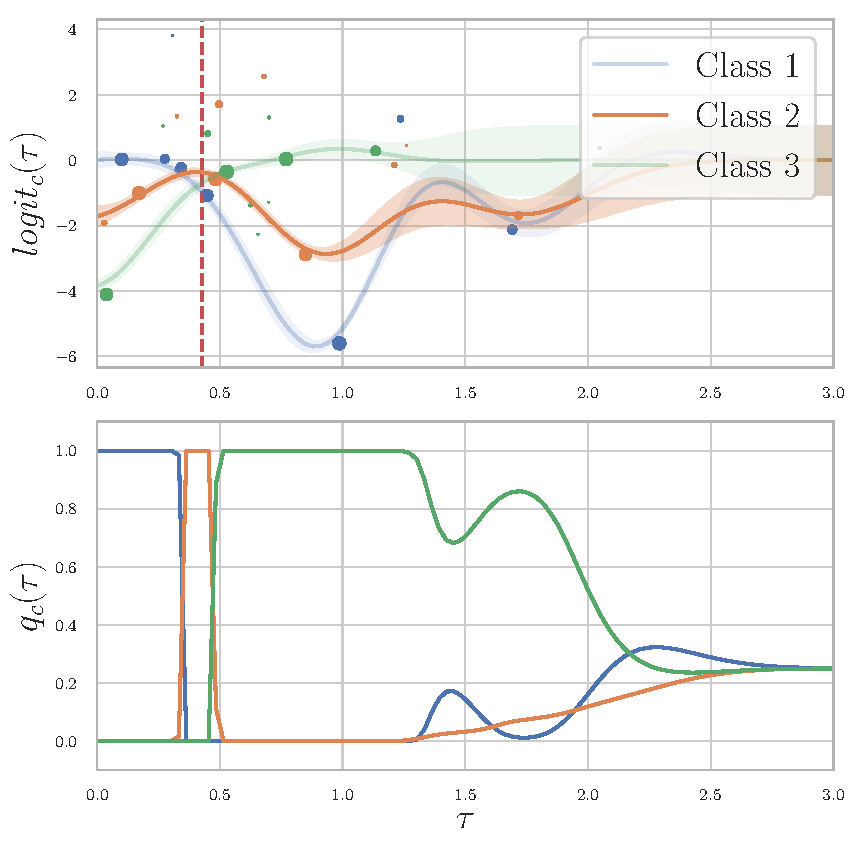
\includegraphics[width=\linewidth]{sections/010_neurips2019/paper/images/shifted-gaussians-gaussian-process.pdf}
        \caption*{\GPModel on 3-G}
    \end{subfigure}
        \begin{subfigure}{.24\textwidth}
        \centering
        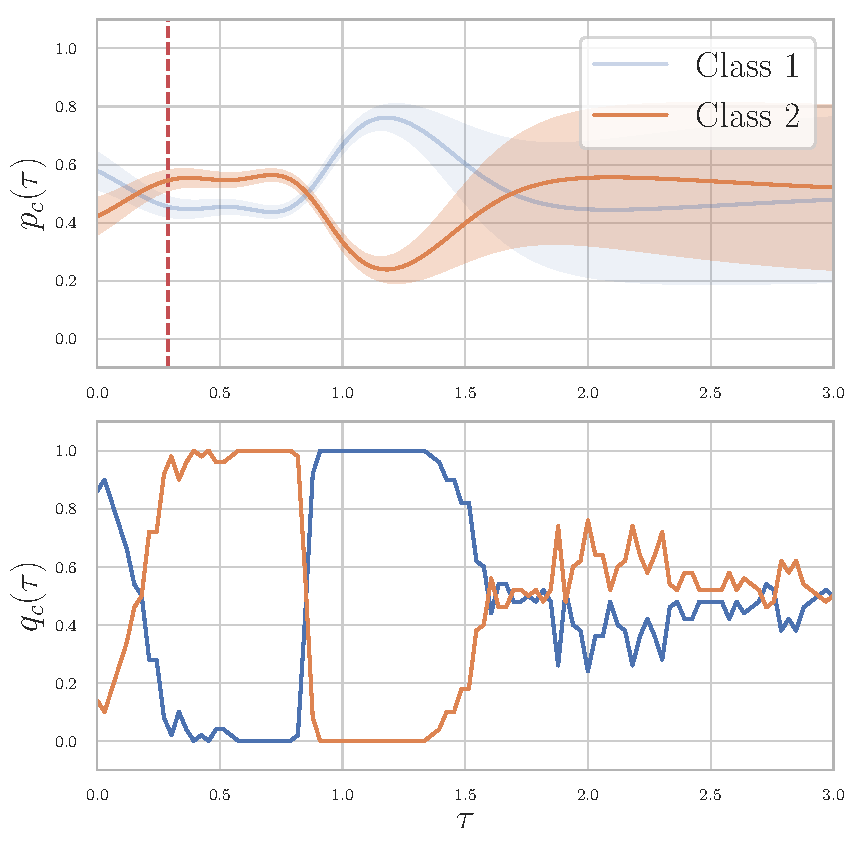
\includegraphics[width=\linewidth]{sections/010_neurips2019/paper/images/shifted-gaussians-multi-dirichlet.pdf}
        \caption*{\DirModel on Multi-G}
    \end{subfigure}
    \begin{subfigure}{.24\textwidth}
        \centering
        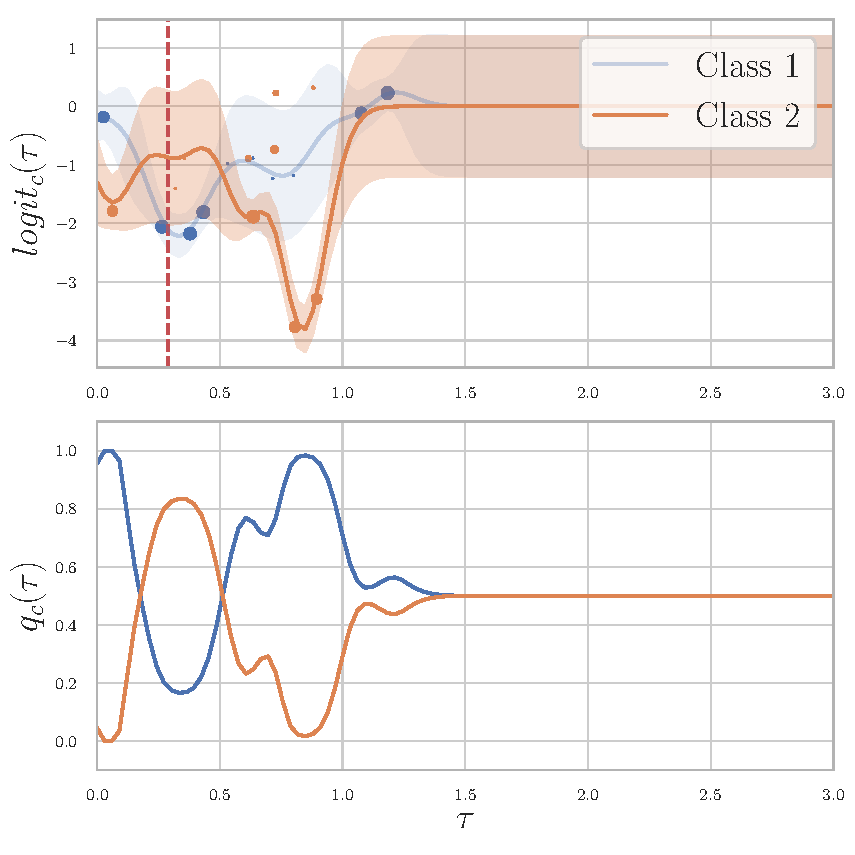
\includegraphics[width=\linewidth]{sections/010_neurips2019/paper/images/shifted-gaussians-multi-gaussian-process.pdf}
        \caption*{\GPModel on Multi-G}
    \end{subfigure}
    \caption{Visualization of the prediction evolution. The red line indicates the true time of the next event for an example sequence. Here, both models predict the orange class, which is correct, and capture the variation of the class distributions over time. Generated points from \GPModel are plotted with the size corresponding to the weight. For predictions in the far future, both models given high uncertainty.}
    \label{fig:visualization}
    \vspace*{-0.5cm}
\end{figure}

\textit{Results.} Both models learn meaningful evolutions of the distribution on the simplex. For the 3-G data, we can distinguish four areas: the first three correspond to the three classes; after that the prediction is uncertain.
% We remark that the model is certain on the first three areas even if the probability of no class is equal to $1$.
% We can also notice the discarding of points in \GPModel.
The Multi-G data shows that both models are able to approximate multimodal evolutions.
